\title{Design Document: CS 378 Lab 2}
\author{Atharva Bendale (22B0901), Nivesh Aggarwal (22B0912), \\Dhvanil Gheewala (22B0923), Vishal Bysani (22B1061)}

\documentclass[11pt]{article}

\usepackage{amsmath}
\usepackage{amssymb}
\usepackage{hyperref}
\usepackage{ulem,graphicx}
\usepackage{subcaption}
\usepackage{gensymb}
\usepackage{tcolorbox}
\usepackage[margin=0.5in]{geometry}
\usepackage{tikz}
\usetikzlibrary{shapes.geometric, arrows}

\tikzstyle{startstop} = [ellipse, minimum width=1.5cm, minimum height=1cm, text centered, draw=black, fill=gray!30]
\tikzstyle{process} = [rectangle, minimum width=1.5cm, minimum height=1cm, text centered, draw=black, fill=orange!30]
\tikzstyle{decision} = [diamond, minimum width=1.5cm, minimum height=1cm, text centered, draw=black, fill=green!30]
\tikzstyle{arrow} = [thick,->,>=stealth]
\begin{document}
% \tcbset{
%   colframe=black,        % Frame color
%   colback=black!10!white, % Background color with transparency
%   boxrule=0.5mm,          % Thickness of the frame
%   arc=3mm,                % Round corners
%   outer arc=3mm,
%   boxsep=5mm,             % Space between the frame and the content
%   breakable,              % Allow breaking across pages
% }
\maketitle
\section{Encoding}
% Preamble, Manchester encoding, etc.
To ensure the proper reception of transmitted signal from the sender's device, we are using the following methods:
\begin{itemize}
    \item \textbf{Multiple-bit Encoding:} We are encoding multiple bits (6 bits) into a single tone. These tones are set uniformly at a gap of 200 Hz starting from 1000 Hz, with a total of 64 frequencies available for encoding data.
    \item \textbf{Special Sequence}: A distinct sequence of bits is used to signal the start of the message. This sequence is $0^{5n}1^n$ (where $n=6$). When the receiver detects at least 5 consecutive tones corresponding to $0^n$ (5 tones of a specific frequency, in this case, 1000 Hz), followed by a tone for $1^n$ (in this case, 13600 Hz), it begins listening for the preamble.

    \item \textbf{Preamble}: The preamble consists of 5 bits representing the length of the original message, encoded in binary. This binary list is then converted into the new base (64) after appending the necessary number of zeros to the right, ensuring that its length is divisible by $\log_2(\text{base})$ (which is 6 in this case).
    \item \textbf{Return to Zero (RZ) Encoding}: We are using the Return to Zero (RZ) encoding scheme to encode the tones. In this scheme, the signal returns to a default frequency of 800 Hz (denoted by \(\psi\)) after each message tone (6 bits). The tones are set in an arithmetic progression, with \texttt{0} at \texttt{1000 Hz}, \texttt{1} at \texttt{1200 Hz}, and \texttt{63} at \texttt{13600 Hz}. This approach ensures that the receiver can clearly distinguish the start and end of each tone. We selected RZ encoding over Manchester encoding because the latter resulted in excessive errors due to uneven tone durations caused by hardware limitations in our speakers.

\end{itemize}
\section{Error Detection}
To detect two bits of error in the transmitted message, our system uses a CRC-k algorithm with Hamming distance 5, this ensures that we could also correct atmost 2 errors.
\begin{tcolorbox}[colback=black!10!white, colframe=black, title=Error Detection Algorithm ]
    \begin{verbatim}
1. Choose a CRC-k polynomial with hamming distance 5, where k is chosen according to the
 message length and use the binary string of the polynomial as divisor
2. Append k 0s to the message and use this as the dividend and store the remainder as CRC 
code C(x) and send the xor of dividend and C(x)
3. When the modified message P(x) is received , our system uses binary polynomial division
with P(x) as dividend and C(x) as divisor. If the remainder is 0 it means that the P(x) is 
error free otherwise it has error\end{verbatim}
\end{tcolorbox}
To further optimise this procedure, we are using as small polynomials as possible corresponding to the message length for reducing the size of transmission as the message length is variable. This information is shared with the receiver with the help of the preamble which has the length encoded in it. \\
All the chosen polynomials have the property that each remainder is mapped to a single transmitted message which has its atmost two bits altered, due to the property of minimum hamming distance being 5. This property makes the polynomials special and ensures the correctness of our algorithm.
\section{Error Correction}
The error correction procedure empolyed is as follows:
\begin{itemize}
    \item If no error is detected then we do nothing (the correctness of this due to the assumption that a maximum of 2 bits can be erroneous)
    \item We iterate over all possible pairs of indices, flip those bits and use our polynomial division subroutine to check if the new message is divisible by the polynomial, if it is then this new message would be the original error free message
    \item If no such pair of indices is found, we iterate over all single bit errors and obtain the corrected message
\end{itemize}
The above procedure outputs the original message if our transmission has no more than 2 bit errors.
\begin{center}
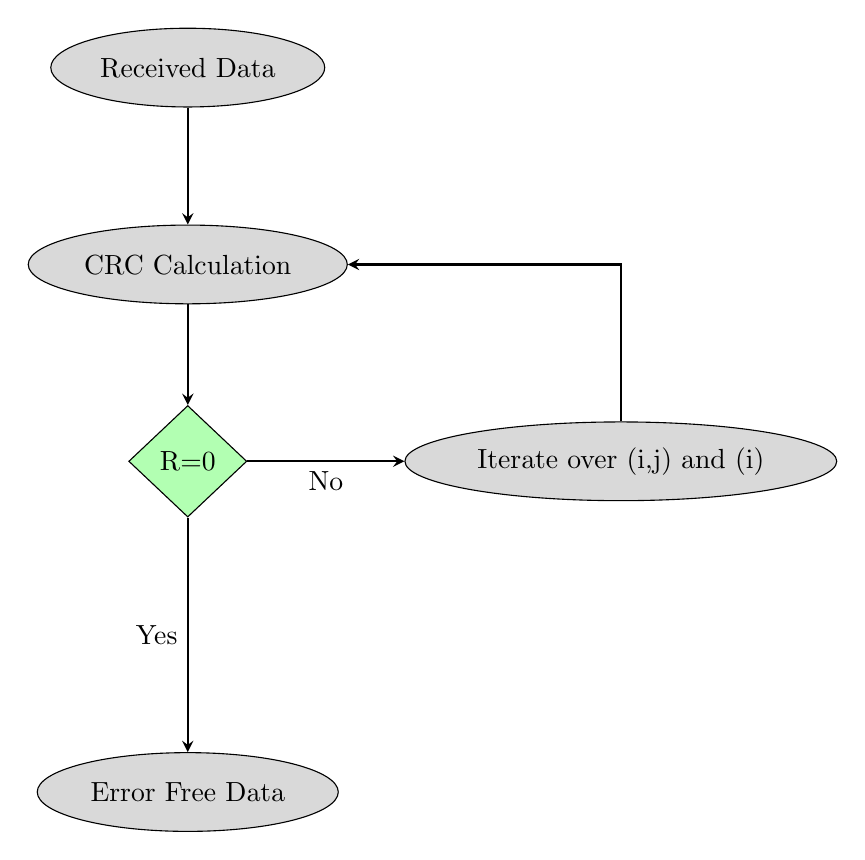
\begin{tikzpicture}[node distance=2.5cm] % Adjust node distance for better spacing

% Nodes
\node (received) [startstop] {Received Data};
\node (crc) [startstop, below of=received] {CRC Calculation};
\node (decision) [decision, below of=crc] {R=0};
\node (errorfree) [startstop, below of=decision, yshift=-1.7cm] {Error Free Data};
\node (ij) [startstop, right of=decision, xshift=3cm]{Iterate over (i,j) and (i)};

% Arrows
\draw [arrow] (received) -- (crc);
\draw [arrow] (crc) -- (decision);
\draw [arrow] (decision) -- node[anchor=east] {Yes} (errorfree);
\draw [arrow] (decision) -- node[anchor=north] {No} (ij);
\draw [arrow] (ij) |- (crc);

\end{tikzpicture}
\end{center}
\noindent Our implementation has support for correction upto triple bit errors too, this can be used via passing an optional argument to the \texttt{encodeCrc} and \texttt{decodeCrc} functions.
\section{Reception}

The reception process in our system focuses on accurately converting the transmitted audio signal back into the original binary sequence. This involves a series of signal processing steps designed to handle noise, detect frequency tones, and decode them into bits. Below, we describe the major components of the reception pipeline.

\subsection{Audio Reception}
The audio signal is captured using the \texttt{receive\_audio()} function, which utilizes the PyAudio library. The system is configured with a sample rate of 44.1 kHz and collects data over a specified duration. We divide the audio stream into frames, with each frame containing 1024 samples. These frames are stored and then concatenated to form the full audio signal as a NumPy array for further processing.
\begin{tcolorbox}[colback=black!10!white, colframe=black]
\begin{verbatim}
audio = pyaudio.PyAudio()
stream = audio.open(format=pyaudio.paFloat32, channels=1, rate=sample_rate, input=True, 
                    frames_per_buffer=1024)
for _ in range(0, int(sample_rate / 1024 * duration)): 
    data = stream.read(1024) 
    frames.append(data)
\end{verbatim}
\end{tcolorbox}
\subsection{Noise Reduction}
To mitigate noise, we run the \texttt{calibrate} function to determine the average noise level in various frequency ranges of the received audio signal. We then use this information to filter out noise from the audio signal by subtracting the average noise level from the signal's power spectrum. This process helps improve the accuracy of frequency detection and bit decoding.
\begin{tcolorbox}[colback=black!10!white, colframe=black]
\begin{verbatim}
stream, audio = self.open_audio_stream(sample_rate)

for _ in range(0, segment_size*white_noise_sample_size, segment_size):
    segment = self.receive_audio(stream, duration, sample_rate)
    freqs, power = signal.welch(segment, sample_rate)
    for i in range(self.base+1):
        self.noise[i] += np.sum(power[(freqs >= self.freq[i]-100) & (freqs <= self.freq[i]
                                                            +100)])
for i in range(self.base+1):
    self.noise[i] = self.noise[i]/white_noise_sample_size
\end{verbatim}
\end{tcolorbox}

\subsection{Frequency-Based Decoding}

The core of the reception mechanism involves detecting the frequency components of the received audio signal to determine the transmitted tone. After segmenting the audio signal into smaller chunks corresponding to each tone's duration (0.15 seconds), we analyze the frequency content of each segment (received using PyAudio) by applying Welch's method, implemented using the \texttt{signal} library from SciPy, for estimating power spectral density.
\begin{tcolorbox}[colback=black!10!white, colframe=black]
    
\begin{verbatim} 
freqs, power = signal.welch(segment, sample_rate)
for i in  range(self.base+1):
    freq_power[i] = np.abs(np.sum(power[(freqs >= self.freq[i]-100) & (freqs <= self.freq[i]
                                                    +100)]) - self.noise[i])
max_ind=np.argmax(freq_power) \end{verbatim}
\end{tcolorbox}

By summing the power within predefined frequency ranges, we can classify each segment according to its corresponding tone, denoted by \( t \in \{0, 1, \ldots, 63\} \cup \{\psi\} \), where \(\psi\) represents the tone corresponding to the default frequency. These tones, excluding \(\psi\), can then be converted into their binary representations to extract the actual bits. This approach enhances the robustness of frequency detection compared to using the Fast Fourier Transform (FFT) alone. Combined with the noise reduction techniques from step 1, it better manages noise and interference in the audio signal, whereas relying solely on FFT's peak might result in detecting noise peaks instead. Additionally, this method does not require consideration of frequency ranges outside the signal's relevant spectrum.




\section{Citations}
% \begin{tcolorbox}
The CRC polynomials used by us are obtained from: \href{https://users.ece.cmu.edu/~koopman/crc/hd5.html}{Best CRC Polynomials}.
% \end{tcolorbox}
\end{document}